\chapter{Betriebsschwingungsanalyse - Campbell-Diagramm}
\label{sec: Hauptkapitel 2}


\section{Aufgabenstellung}
%=========================
    % Grundziel
    %----------
    Ziel dieser Laboraufgabe ist das Durchführen einer Betriebsschwingungsanalyse
    mit anschließender Erstellung eines Campbell-Diagramms. Der Motor des
    Modellflugzeugs soll dabei von einem Elektromotor ohne Verdichtung
    geschleppt werden. Das Schwingungssignal soll an einem bestimmten Punkt der
    Tragfläche abgenommen werden.
%================================================================================

\section{Versuchsaufbau}
%=======================
    % Verwendete Geräte
    %------------------
    Für diesen Versuchsaufbau wurden folgende Geräte verwendet:

    \begin{table}[H]
        \centering
        \begin{tabular}{|l|l|p{6cm}|}
            \hline
            \textbf{Gerät}  &   \textbf{Gerätename}   &   \textbf{Sensordaten} \\
            \hline \hline
            CompaqDAQ Chassis & cDAQ-9171 & hostpowered \\
            \hline
            CompaqDAQ Input Modul & NI 9234 & 4 Kanäle, ±5 V, 51,2 kS/s pro Kanal, 24 bit-IEPE  \\
            \hline
            CompaqDAQ Output Modul & NI 9201 & 8 Kanälen, 500 kS/s, 12 bit, ±10 V   \\
            \hline
            Beschleunigungssensor & 8702B25 & Kistler, Piezo, ±25g, 1Hz-9kHz, UniAx, 169 mV/g  \\
            \hline
            Beschleunigungssensor & 8702B25 & Kistler, Piezo, ±50g, 0.5Hz-5kHz, UniAx, 96.5 mV/g  \\
            \hline
            Elektromotor & - & FH-Wels, max. 12 V \\
            \hline
        \end{tabular}
        \caption{Geräteliste - Betriebsschwingungsanalyse}
        \label{tab: Geräteliste_BSA}
    \end{table}

    % Sensorplatzierung
    %------------------
    \noindent
    Obwohl nur ein Sensorsignal ausgewertet werden muss, werden 4
    Beschleunigungssensoren am vorderen Tragflügel platziert.
    Somit kann mit einem Aufbau und einer Messung sowohl die Aufgabe von Kapitel
    \ref{sec: Hauptkapitel 2} und Kaptiel \ref{sec: Hauptkapitel 3}
    abgewickelt werden. Die Beschleunigungssensoren werden an Punkten 1, 2, 4 und
    5 rot platziert (siehe Abbildung \ref{fig: Sensorpos_BSA}). Im Zuge von
    Kapitel \ref{sec: Hauptkapitel 2} wird der Messpunkt 5 rot verwendet.

    % Bild - Sensorplatzierung BSA
    %-----------------------------
    \begin{figure}[H]
        \centering
        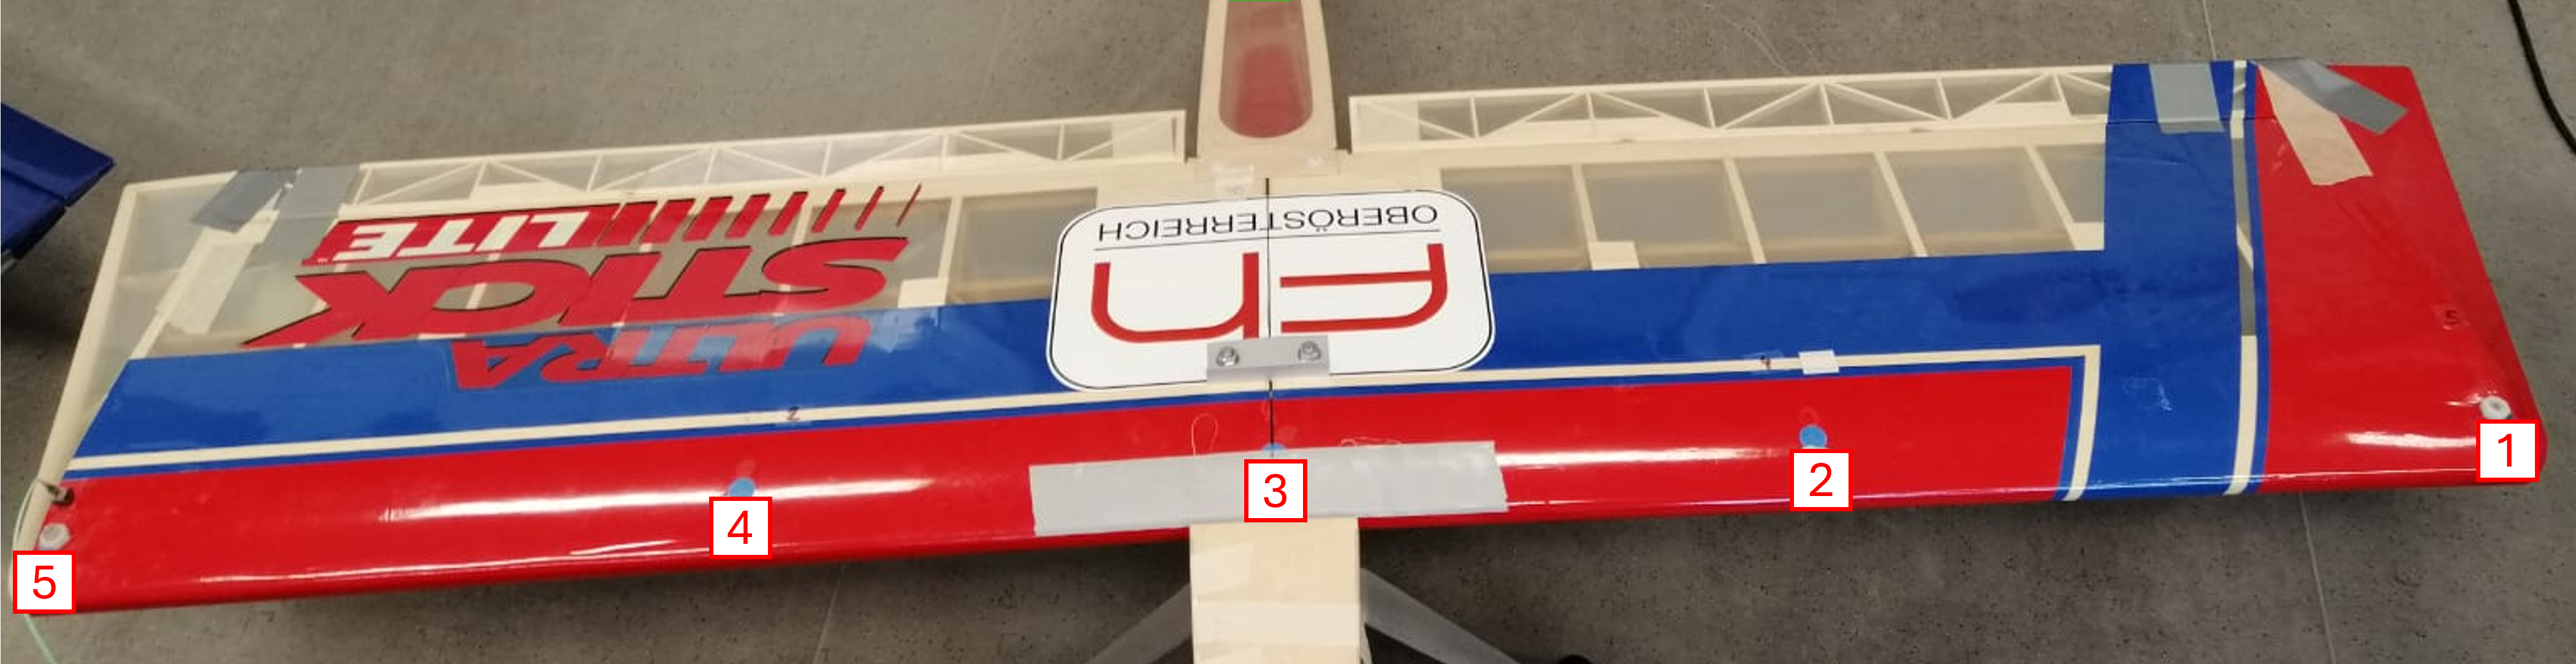
\includegraphics[width=0.9\textwidth]{BSA_Sensorpositionen.png}
        \caption{Sensorpositionen BSA}
        \label{fig: Sensorpos_BSA}
    \end{figure}
    %----------------------------------------------------------------------------

    % Fixierung Flieger
    %------------------
    \noindent
    Damit der Modellflieger bei den Messungen nicht durch die Anregung
    verschoben wird, wird er am Boden fixiert. Dazu werden behelfsmäßige Keile mit
    Klebeband am Boden bei den Rädern befestigt.
    \\
    %----------------------------------------------------------------------------

    % Messung mit Motor
    %------------------
    \noindent
    Bevor nun die Betriebsschwingungsanalyse durchgeführt werden kann, wird der
    Motor des Modellflugzeugs mit etwas Öl geschmiert. Dann wird der Elektromotor
    an die Welle zum Übertragen des Drehmoments angesetzt. Nun kann die Messung
    gestartet werden. Dabei wird der Elektromotor langsam mit einer Rampe von einer
    Spannung von 0 [V] auf 5 [V] beschleunigt. Während der Messung wird der
    Elektromotor in der Hand gehalten.
    \\
    %----------------------------------------------------------------------------

    % Drehzahlmessung
    %----------------
    \noindent
    Da das Ziel dieser Laboraufgabe die Erstellung eines Campbell-Diagramms ist,
    muss zusätzlich zum Beschleugingungssignal auch die Drehzahl des Motors
    aufgenommen werden. Dazu wird ein Beschleunigungssensor am Motorgehäuse
    angebracht und der Elektromotor mit einer konstanten Spannung betrieben. Da
    der Motor eine gewisse Unwucht aufweist, ist in regelmäßigen Abständen eine
    Spitze im Beschleugingungssignal zu sehen. Dadurch kann auf die Drehzahl
    rückgeschlossen werden. Anschließend wird eine 2. Messung mit einer höheren
    Spannung durchgeführt und erneut die Drehzahl bestimmt. Unter Annahme eines
    linearen Zusammenhangs zwischen Spannung und Drehzahl kann nun eine Funktion
    der Drehzahl in Abhängigkeit der Spannung gefunden werden. Die durchgeführten
    Messungen sind in Tabelle \ref{tab: Drehzahlmessung} zu sehen.
    %----------------------------------------------------------------------------

    % Tabelle - Drehzahlmessung
    %--------------------------
    \begin{table}[H]
        \centering
        \begin{tabular}{|c|c|c|}
            \hline
            \textbf{Spannung [V]} & \textbf{Frequenz [HZ]} & \textbf{Drehzahl [U/min]} \\
            \hline \hline
            1   &   8   &   480 \\
            \hline
            2   &   17.5    &   1050 \\
            \hline
            4   &   36.6    &   2196 \\
            \hline
        \end{tabular}
        \caption{Messungen zur Bestimmung der Drehzahl}
        \label{tab: Drehzahlmessung}
    \end{table}
    %----------------------------------------------------------------------------

    % Erklärung - Centerpoint
    %------------------------
    \noindent
    Wie in Tabelle \ref{tab: Drehzahlmessung} zu sehen ist, wurde auch eine 3.
    Messung durchgeführt. Diese dient als Centerpoint-Messung und soll
    überprüfen, ob auch wirklich ein linearer Zusammenhang vorliegt. In Abbildung
    \ref{fig: Drehzahlmessung} sind die 3 Messungen in einem Diagramm dargestellt.

    % Bild - Drehzahlmessung
    %-----------------------
    \begin{figure}[H]
        \centering
        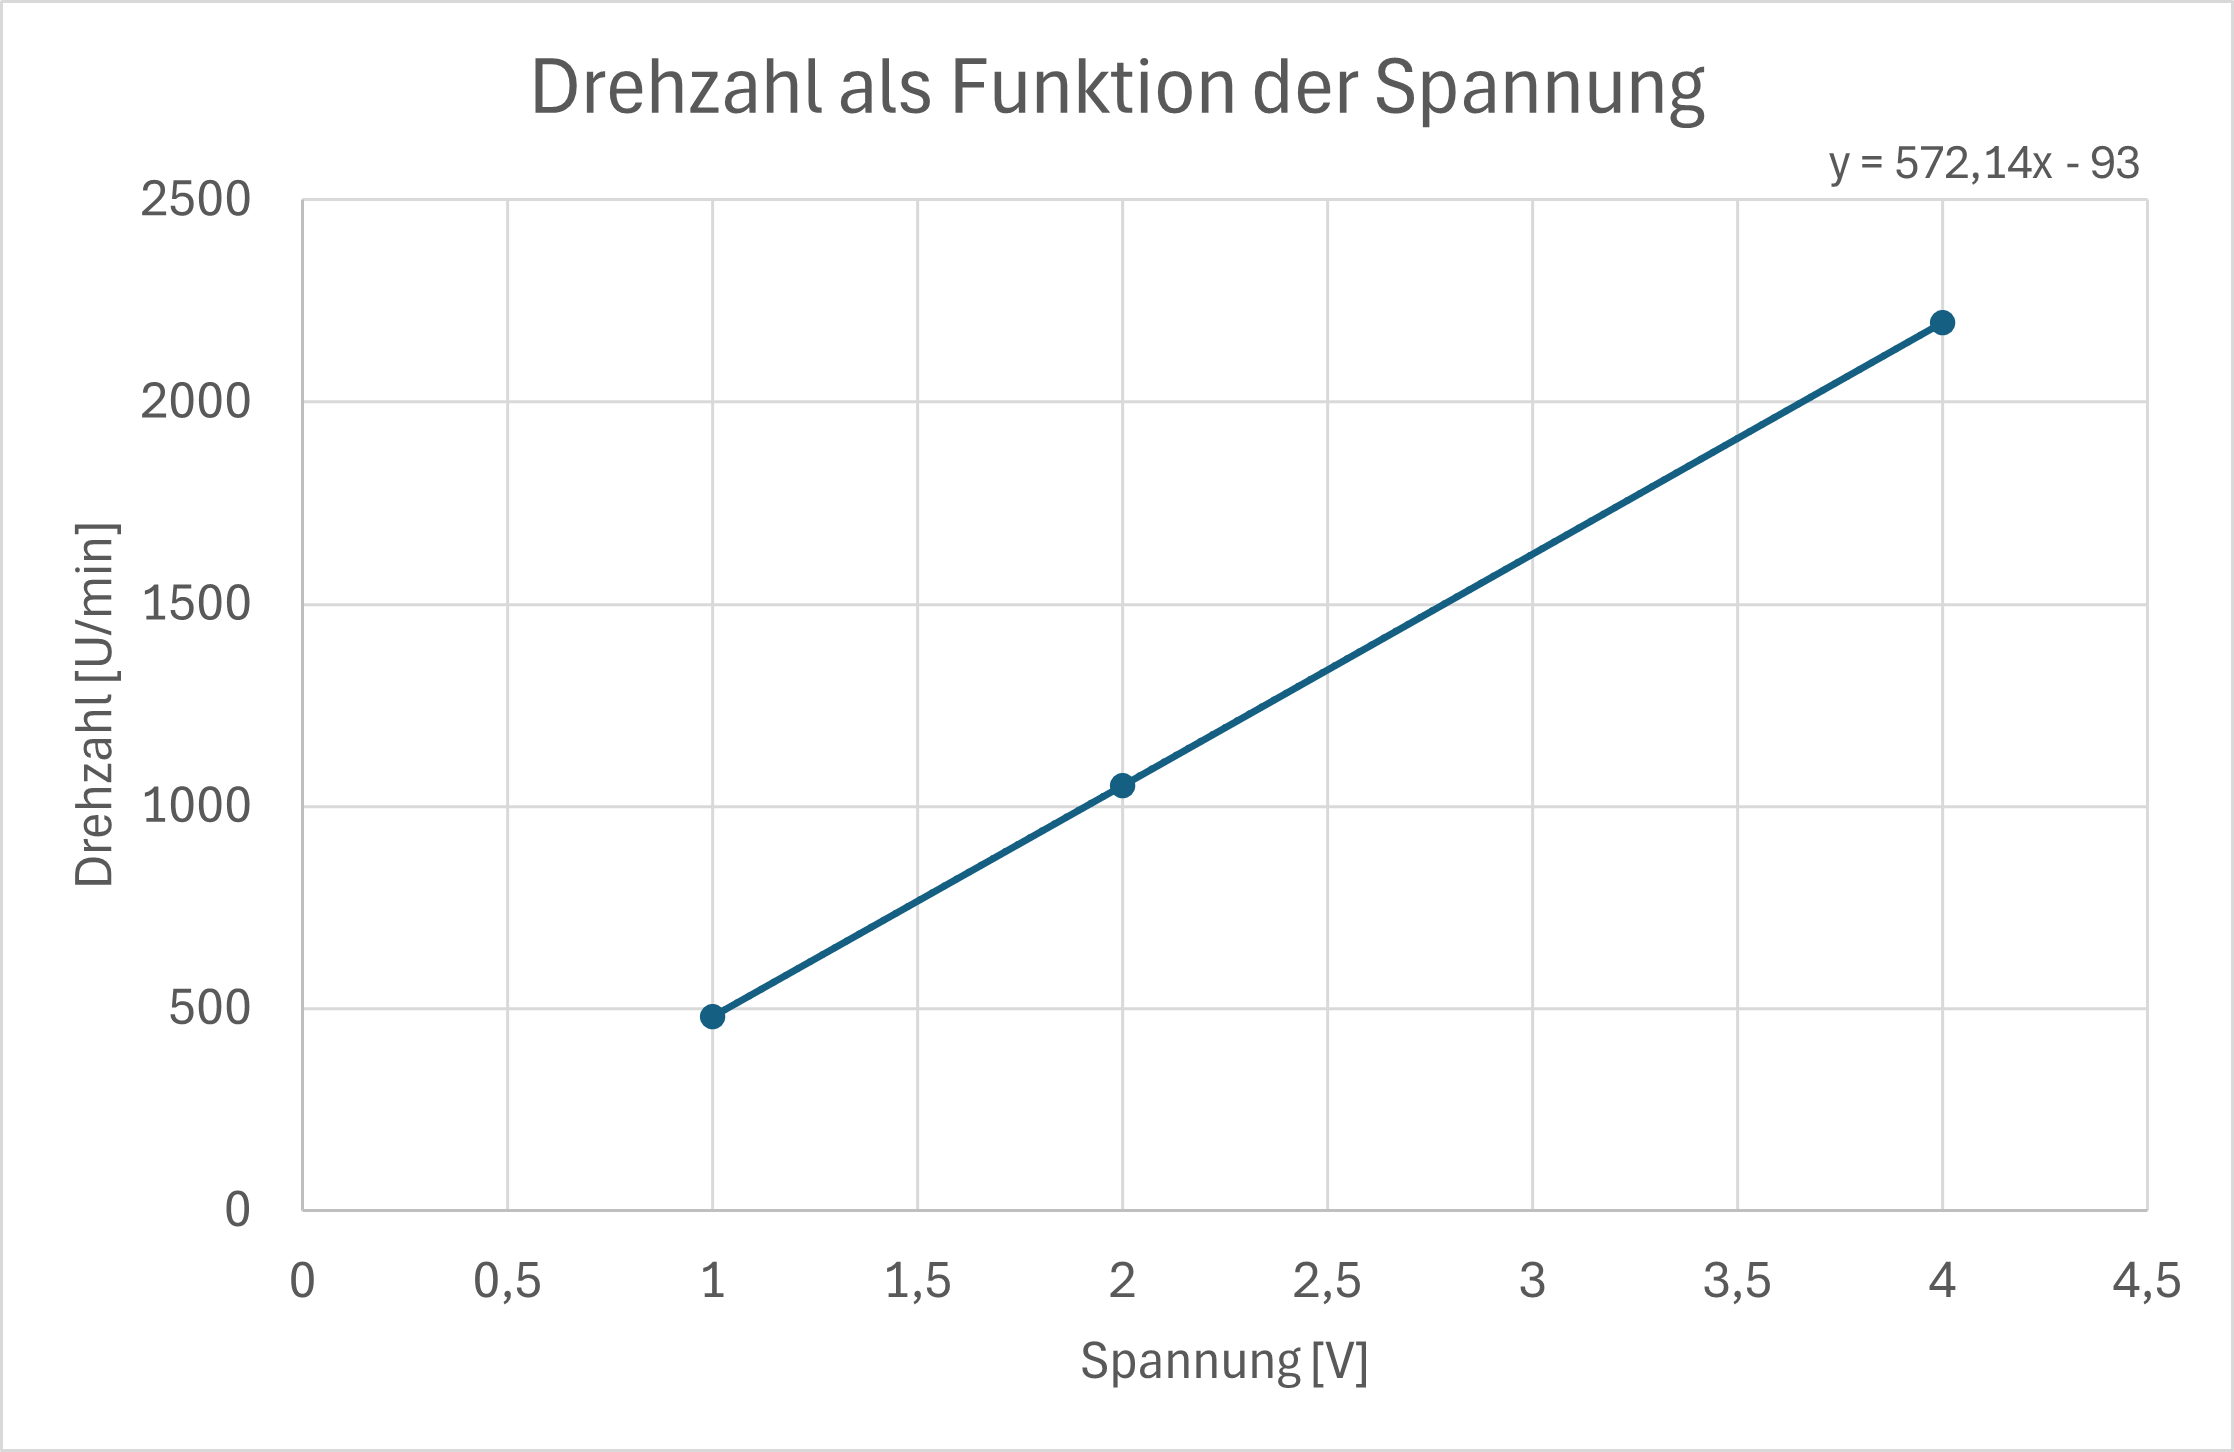
\includegraphics[width=0.7\textwidth]{Drehzahlmessung.png}
        \caption{Zusammenhang zwischen Spannung und Drehzahl}
        \label{fig: Drehzahlmessung}
    \end{figure}

    % Bildbeschreibung
    %-----------------
    \noindent
    Wie in Abbildung \ref{fig: Drehzahlmessung} gut zu sehen ist, verhält sich
    der Zusammenhang zwischen Spannung und Drehzahl wirklich linear. Auch der
    Centerpoint liegt schön auf der Linie. Somit kann folgender Zusammenhang
    angenommen werden:

    % Formel - Zus. zw. Spg. und Drehzahl
    %------------------------------------
    \begin{equation*}
        n = 572.14 \cdot U - 93
    \end{equation*}
%================================================================================

\section{Ergebnisse}
%===================
    % Campbell-Diagramm
    %------------------
    Mit den Daten aus den Versuchen kann nun über ein Python-Skript ein
    Campbell-Diagramm erstellt werden (siehe Anhang \ref{sec: Anhang_BSA}). Das
    Skript erstellt für alle 4 Messpunkte ein Diagramm, allerdings wird in der
    Auswertung hier nur der Messpunkt \glqq 5 rot\grqq \hspace{0.05cm} betrachet.
    Das zugehörige Campbell-Diagramm ist in Abbildung
    \ref{fig: Campbell_Diagramm} dargestellt.

    % Bild - Campbell-Diagramm
    %-------------------------
    \begin{figure}[H]
        \centering
        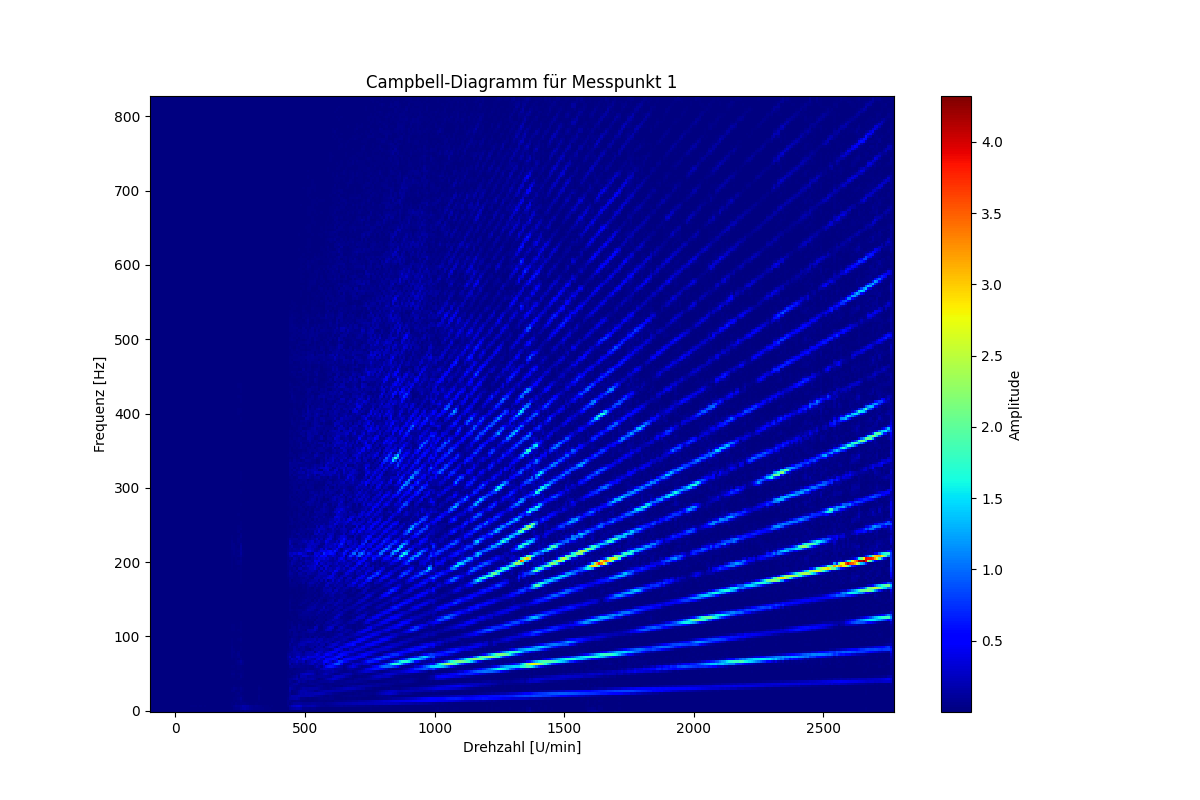
\includegraphics[width=1.2\textwidth]{Campbell_Diagramm_MP1.png}
        \caption{Campbell-Diagramm Messpunkt \glqq 5 rot\grqq}
        \label{fig: Campbell_Diagramm}
    \end{figure}
    %----------------------------------------------------------------------------

    % Interpretation
    %---------------
    \noindent
    Aus Abbildung \ref{fig: Campbell_Diagramm} geht hervor, dass die meisten der
    Amplitudenausschläge lastabhängig sind. Allerdings sieht es so aus, als ob bei
    etwa 60 [Hz] tatsächlich ein Schwingungsmode liegt. Des Weiteren dürfte auch
    bei zirka 215 [Hz] ein Schwingungsmode liegen. Diese Annahmen decken sich
    auch ganz gut mit dem Amplitudenplot aus Laboraufgabe 1. Wird hier die
    x-Achse weiter angezeigt als bis 60 [Hz], können die beiden oben entdeckten
    Moden auch gesehen werden. Dies ist in Abbildung
    \ref{fig: Modevergleich_CB_EMA} dargestellt.

    % Bild - Modevergleich
    %---------------------
    \begin{figure}[H]
        \centering
        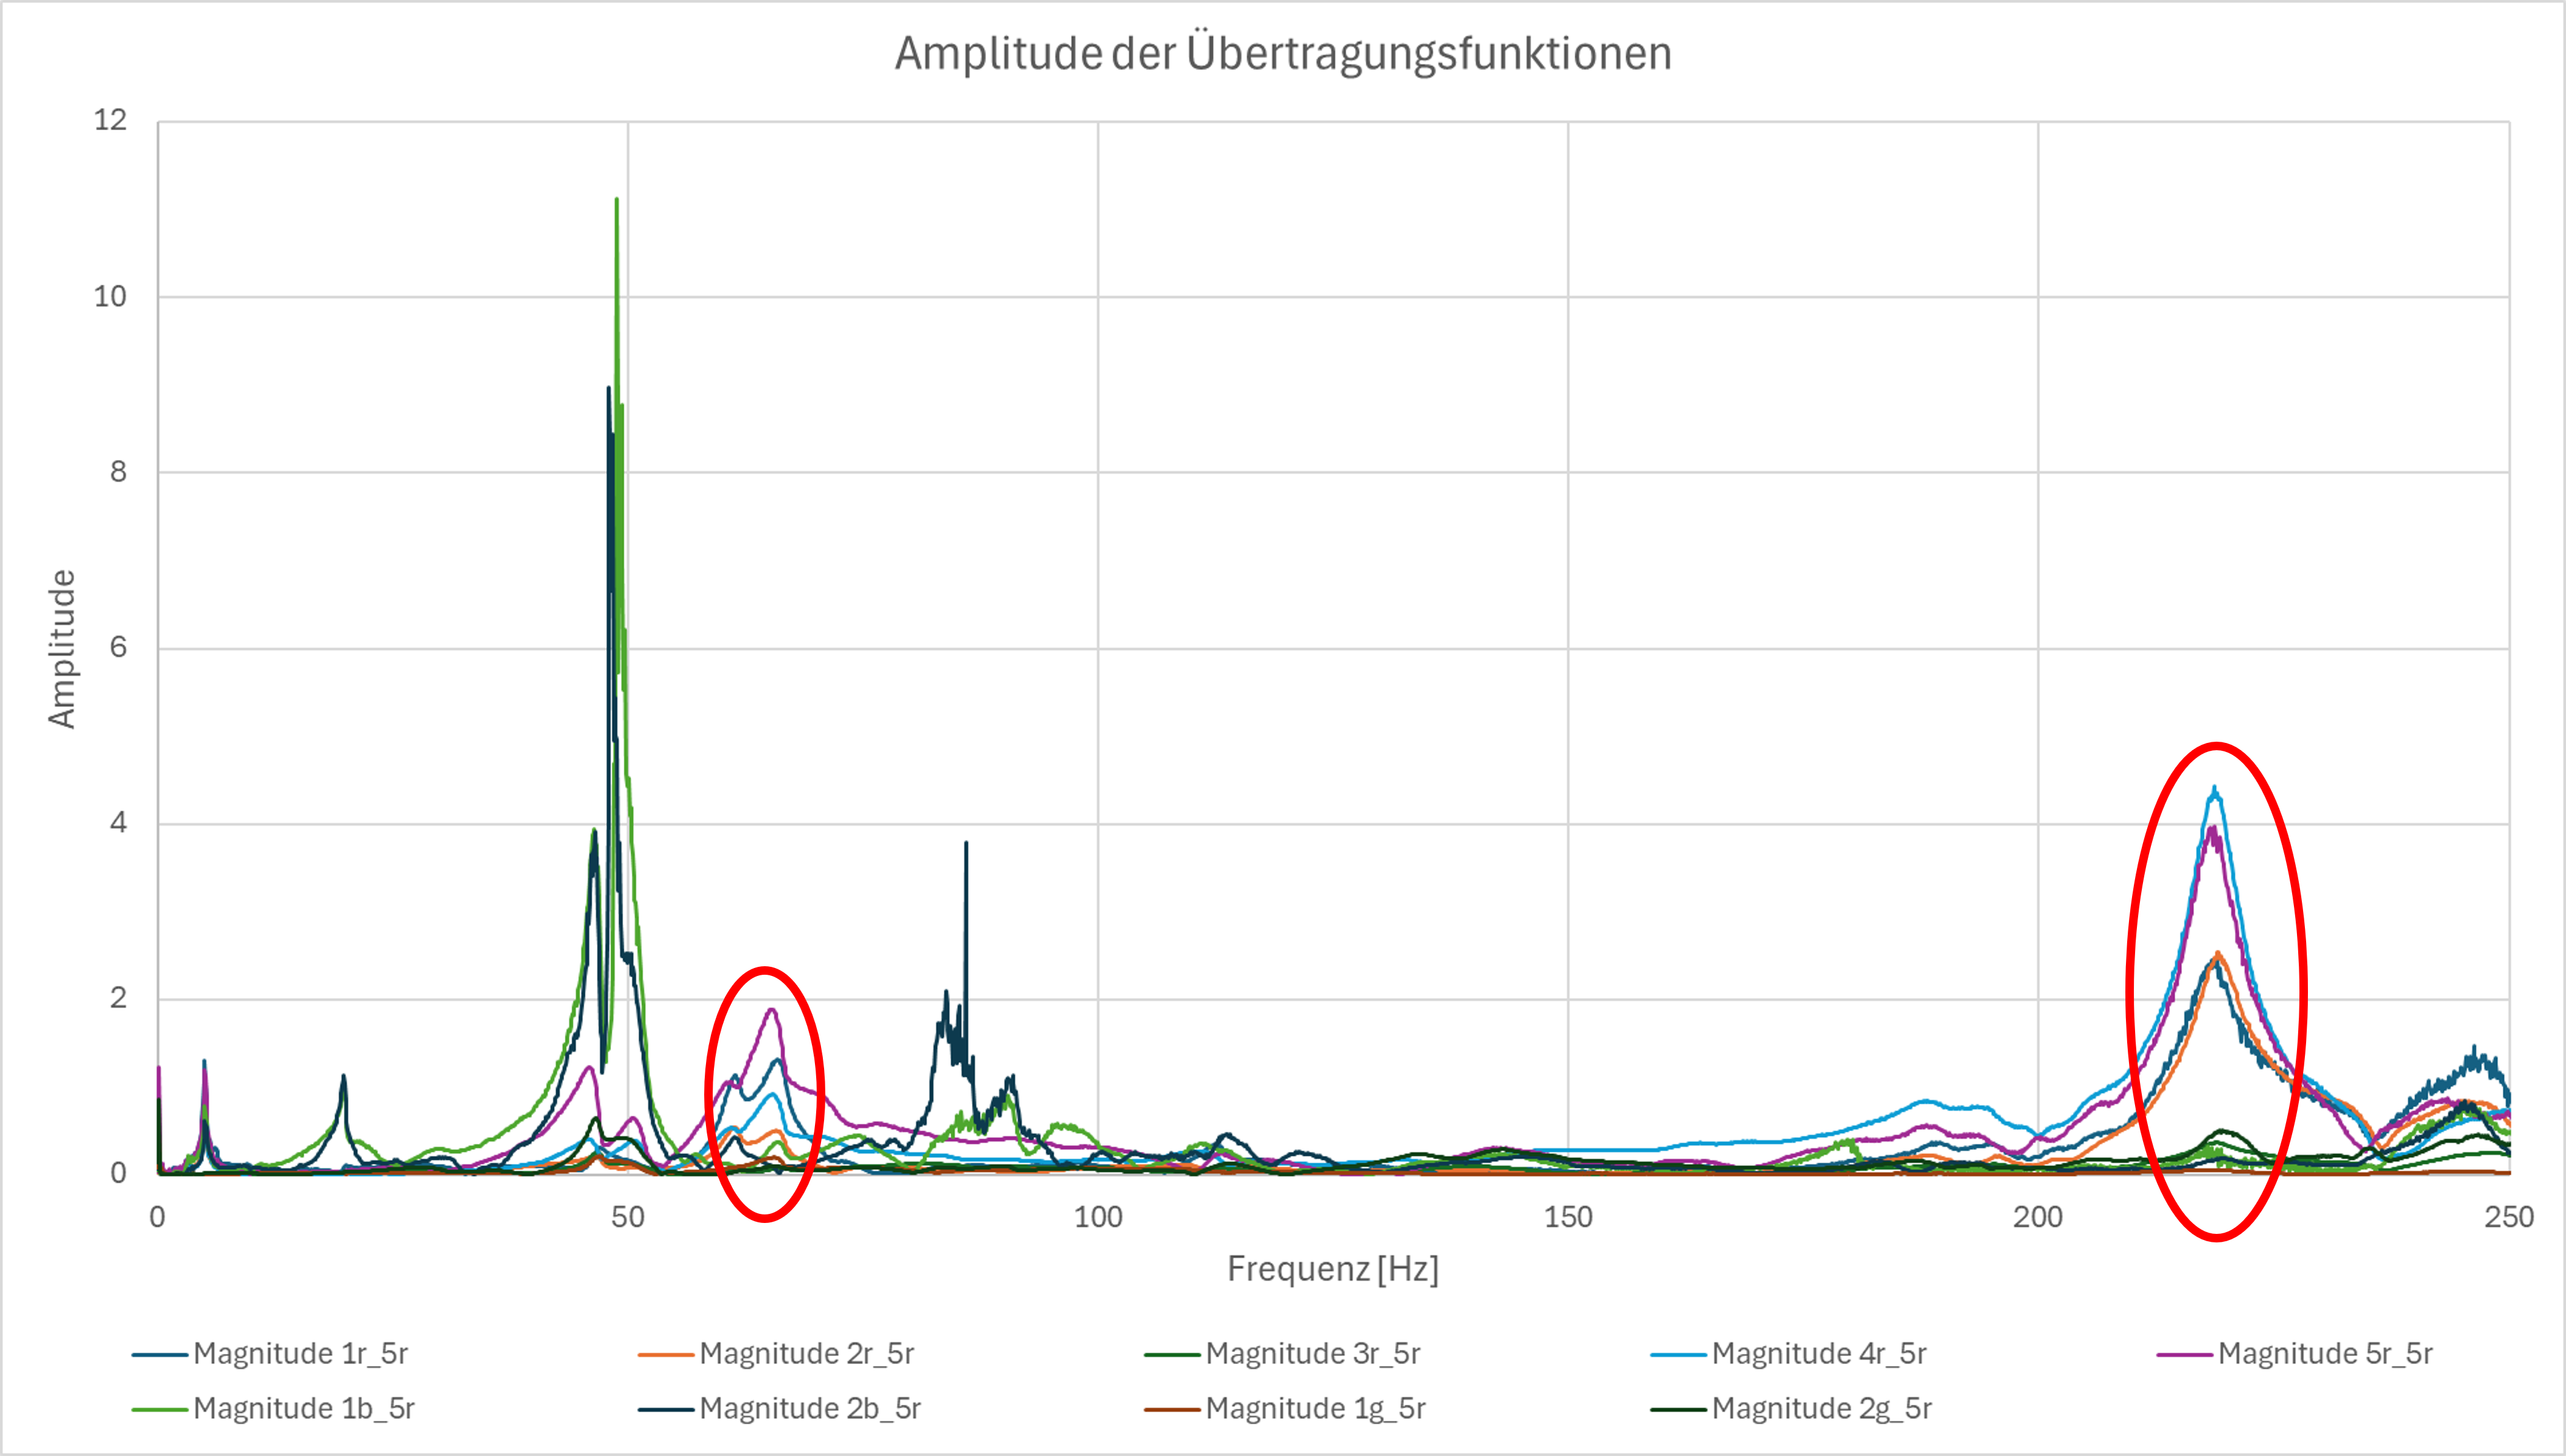
\includegraphics[width=1\textwidth]{Moden_aus_CB_Diagramm.png}
        \caption{Moden des Campbell-Diagramms verglichen mit EMA}
        \label{fig: Modevergleich_CB_EMA}
    \end{figure}


